\documentclass[a4paper, twocolumn]{article}
\setlength{\columnsep}{40pt}
\usepackage{graphicx} 
\usepackage[a4paper,margin=0.5in]{geometry}
\usepackage{amsmath}

\begin{document}

\title{Data Visualization on the Titanic Dataset}
\author{Jawadul Chowdhury}
\date{\today}
\maketitle

\section{Introduction}
The Titanic was a British passenger ship that sank in the Atlantic Ocean on April 15, 1912. The ship had struck an 
iceberg on its maiden voyage from Southampton, England to New York City. 

We use exploratory data analysis on the titanic dataset, using different visualizatoin tehcniques as well as
determining which features are should be included in a machine learning model.

\section{Dataset Description}
When examining the dataset, there are a total of 16 features. Such variables are listed as follows:

\begin{itemize}
    \item \texttt{PassengerId}: The ID of the passenger. This is a discrete numerical data type as the difference
     between units is constant.
    \item \texttt{Survived}: Whether the passenger survived or not.This is a nominal binary categorical data type 
    as there is no order information. 0 means passenger didn't survive and and 1 means passenger did survive.
    \item \texttt{Pclass}: This is the passenger class. It is a ordinal categorical data type, as 1 means 1st ticket 
    class and so on for 2 and 3, to identify passenger class.
    \item \texttt{Name}: The name of the passenger. This is a  nominal categorical data type, as the names of the 
    passenger have no order information.
    \item \texttt{Sex}: This is the sex of the passenger. This is a nominal categorical data type,as genders can't be 
    ordered and is rather binary.
    \item \texttt{Age}: Age of the Passenger. This is a continuous numerical data type, as the difference between 
    units is constant and can be counted.
    \item \texttt{SibSp}: Number of Siblings / Spouses of the passenger. It is a discrete numerical data type as it 
    can be counted and has a constant difference between units.
    \item \texttt{Parch}: Number of Parents / Children abroad the Titanic. It is a discrete numerical data type, as 
    it can be counted and can only take certain values.
    \item \texttt{Ticket}: This is the ticket number. This is a  nominal categorical data type as there is no ordering 
    information.
    \item \texttt{Fare}: This is the passenger fare. This is a ratio numerical data type as there is a true zero, 
    where zero means that the passenger has not paid any fare.
    \item \texttt{Cabin}: This is the cabin number of the passenger. It is a nominal categorical data type as there 
    is no order information bur rather a quantitvate classifcation.
    \item \texttt{Embarked}: This is the port where the passenger embarked. C is Cherbourg, Q is Queenstown and S 
    is Southampton. This is a categorical nominal data type as there is no order information and has quantitative 
    classification.
    \item \texttt{Age\_fill\_mean}: This is a copy of the Age column but the blanks have been filled in with the mean.
    This is a ratio numerical data type, because there are  fractional values and has a true zero point.
    \item \texttt{Age\_fill\_median}: This is a copy of the Age column but the blanks have been filled in with the
    median. This is a discrete numerical data type because the age is defined to be continuous numerical.
    \item \texttt{Age\_fill\_mode}: This is a copy of the Age column but the blanks have been filled in with the mode.
    This is a discrete numerical data type, because the age is defined to be continuous numerical.
    \item \texttt{Age\_fill\_knn}: This is a copy of the Age column but the blanks have been filled in with the mean.
    This is a ratio numerical data type, because there are fractional values and has a true zero point.
\end{itemize}


\section{Observing Visual Graphs}
Visual Graphs can be of different types. For this paper, we look at the following for each visualization:
\begin{enumerate}
    \item Box Plots: The Median \& Interquartile Range Mark
    \item Heat Map: The Color Intensity
    \item Violin Plot: The Median
\end{enumerate}

\section{Data Visualization \& Analysis}
Now, we move on to visualizting some of the variables we have in the Titanic dataset against the \texttt{Survived}
variable. We also look for any predictive relationships using the plots.

\subsection{Fare vs Survived}
In order to determine a appropriate plot type, we need to identify the type of data. We know that the 
\texttt{Survived} variable is binary and categorical, and we know that \texttt{Fare} is a ratio numerical data type.
For this application, it would be best to use a box plot since we're dealing with categorical / numerical data, as 
shown in Figure 1.

In this visualization, we can see that the medians of both the box plots are close. This suggests that both the groups
have similar tendencies, hence it doesn't strongly differentiate survivors from non-survivors. If the medians are
different, this means that the variable has a predictive power, which is otherwise the case. We can also look at the
overlapping of the IQR between both plots. Since they overlap a lot, this means a weaker relationship. As a result,
this variable isn't related to the \texttt{Survived} variable.

\begin{figure}[h!] 
    \centering
    \noindent
    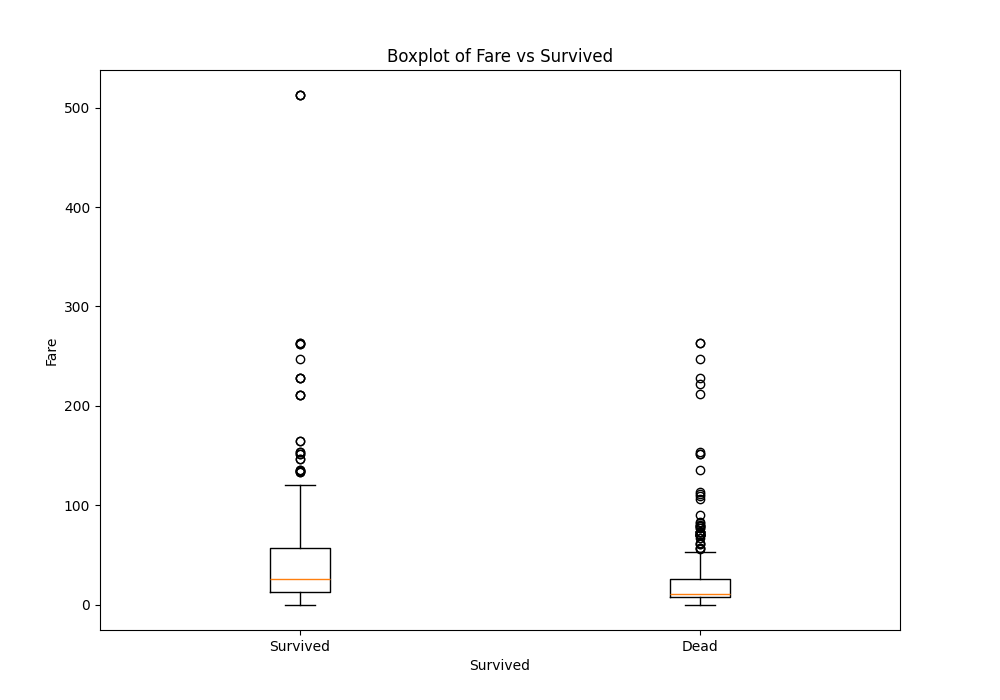
\includegraphics[width=\columnwidth]{C:/GitHub/DataScience/wk_03/plots/BoxPlotFareSurvived.png}  
    \caption{Box Plot of Fare vs Survived} 
\end{figure}

\subsection{Sex vs Survived}
Next up, we now plot the \texttt{Sex} variable against \texttt{Survived} variable. We know that the \texttt{Sex}
variable is a categorical variable, which uses male and female. We also have the survived variable which is also
categorical as discussed previously. For this application, we can use a Heat Map since we're dealing with categorical
/ categorical data as shown in Figure 2.

In this visualization, we can see different intensities of the same color on the heatmap. It can be seen that there
is a deep blue color between females and being able to suvived and also males and not surviving. Such a deep blue
color is shows a predictive relationship. We can also confirm this by looking at the value of the probability, which is greater than 0.7, hence suggesting a 
strong likelihood and predictive relationship. As a result, this variable is related to the \texttt{Survived} variable.

\begin{figure}[h!] 
    \centering
    \noindent
    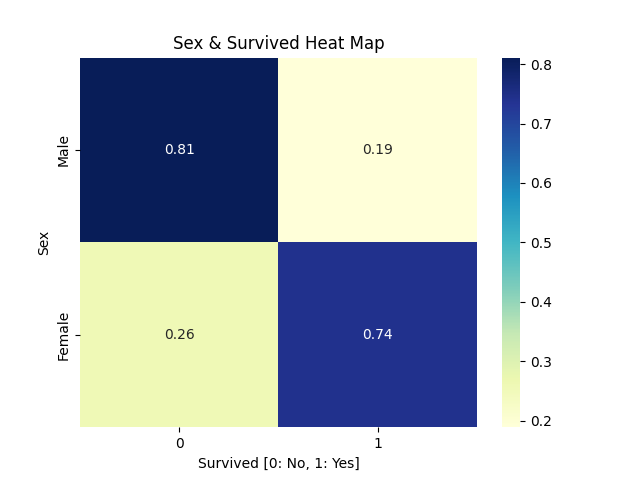
\includegraphics[width=\columnwidth]{C:/GitHub/DataScience/wk_03/plots/HeatMapSexSurvived.png}  
    \caption{Heat Map of Sex vs Survived} 
\end{figure}

\subsection{Sibling / Spouse vs Survived}
Next up, we now plot the \texttt{SibSp} variable against the \texttt{Survived} variable. We know that the
\texttt{SibSp} variable is a discrete numerical data type, as it can be counted. As a result, since we're plotting
a numerical data type against a categorical data type, we can use a bot plot to best represent this numerical 
/ categorical data as shown in Figure 3.

In this visualization, we can see that the median is exactly the same in both box plots. This suggests that both
groups have similar central tendencies. However, this is absolutely no predictive relationship at all. We can also
confirm by looking at the IQR, which appear to overlap perfectly. Such a large overlap reduces the predictive power.
As a result, this variable isn't related to the \texttt{Survived} variable.

\begin{figure}[h!] 
    \centering
    \noindent
    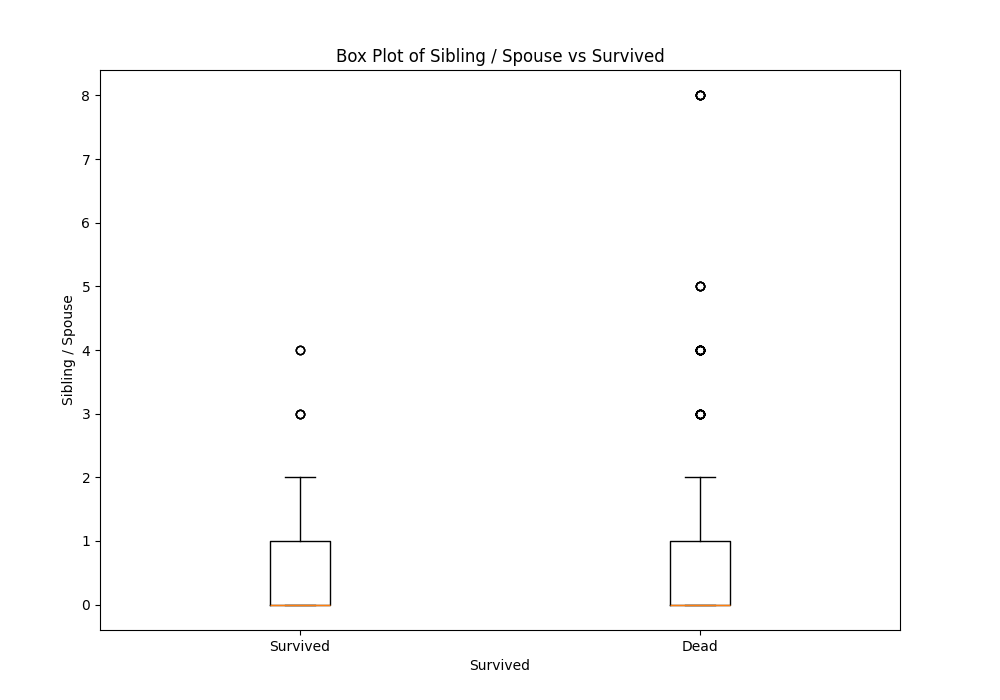
\includegraphics[width=\columnwidth]{C:/GitHub/DataScience/wk_03/plots/BoxPlotSibSpSurvived.png}  
    \caption{Heat Map of Sibling / Spouse vs Survived} 
\end{figure}

\subsection{Parent / Children vs Survived}
Moreover, we now plot the \texttt{Parch} variable against the \texttt{Survived} variable. We know that the 
\texttt{Parch} variable is a discrete numerical data type, as it can be counted. As a result, since we're plotting
a numerical data type against a categorical data type, we can use a bot plot to best represent this as shown in 
Figure 4.

In this visualization, we can see that the median values are exactly the same in both the box plots. This suggests
that both the groups have similar tendencies. This is a strong indication that there is no predictive relationship.
Furthermore, there is no overlap between the IQR of both the box plots, which strengthens the claim. As a result,
this variable isn't related to the \texttt{Survived} variable.

\begin{figure}[h!] 
    \centering
    \noindent
    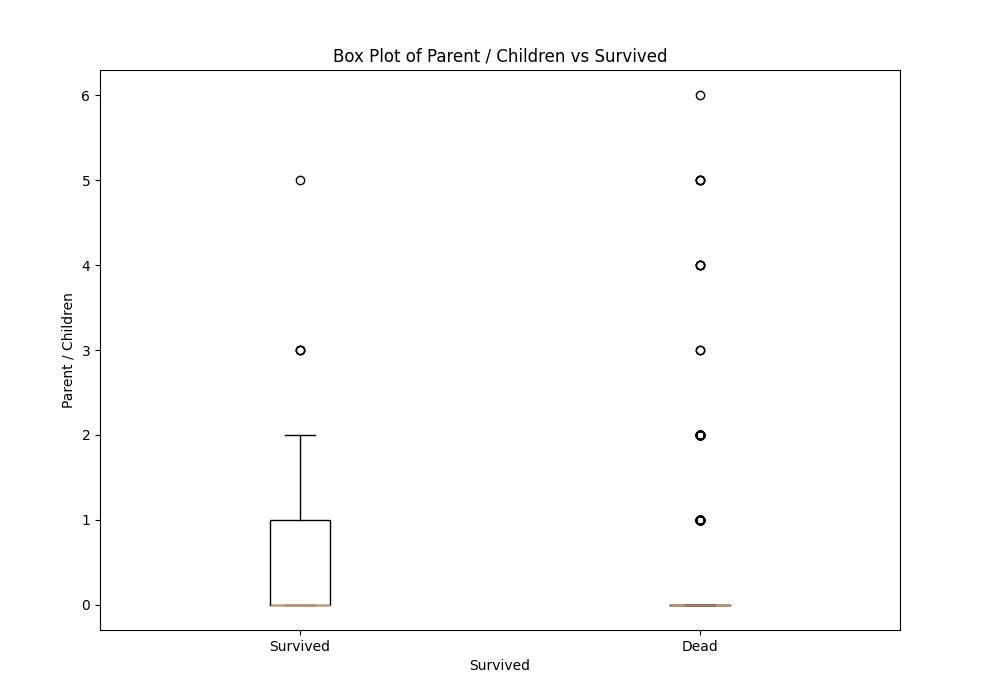
\includegraphics[width=\columnwidth]{C:/GitHub/DataScience/wk_03/plots/BoxPlotParchSurvived.png}  
    \caption{Box Plot of Parent / Children vs Survived} 
\end{figure}


\subsection{Embarked vs Survived}
Moving on, we now plot the \texttt{Embarked} variable against the \texttt{Survived} variable. We know that the 
\texttt{Embarked} variable is a categorical data type, and since we're plotting the a categorical data type against
a categorical data type, we can then use a heat map to best represent this as shown in Figure 5.

In this visualization, we can see a heat map, in which the higher the intensity of the color on the heatmap, the 
stronger the predictive relationship between them. It is clear to see that passengers who embarked from Southamptona
and Queenstown are more likely to not have survived. This is backed by the variable measure of probability, which
is greater than 0.6. As a result, such variables mentioned have a strong relationship with the \texttt{Survived}
variable.

\begin{figure}[h!] 
    \centering
    \noindent
    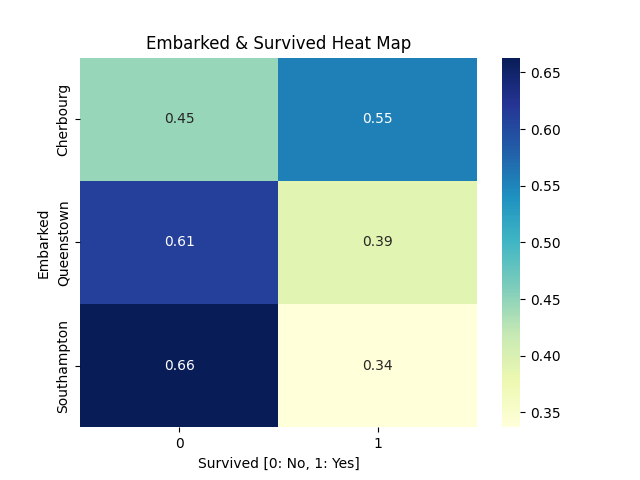
\includegraphics[width=\columnwidth]{C:/GitHub/DataScience/wk_03/plots/HeatMapEmbarkedSurvived.png}  
    \caption{Heat Map of Embarked vs Survived} 
\end{figure}

\subsection{Passenger Class vs Survived}
Next, we now plot the \texttt{Pclass} variable against the \texttt{Survived} variable. We know that the 
\texttt{Pclass} variable is a categorical data type, and since we're plotting the a categorical data type against
a categorical data type, we can then use a heat map to best represent this as shown in Figure 6.

In this visualization, we can see a heat map, in which the higher the intensity of the color on the heatmap, the 
stronger the predictive relationship between them. It is clear to see that passengers of class 3 are more likely 
to not survive and that passengers of class 1 are more likely to survive. And such observations are backed by 
the numerical probabilities which are higher than 0.6. As a result, such variables mentioned have a strong 
relationship with the \texttt{Survived} variable.

\begin{figure}[h!] 
    \centering
    \noindent
    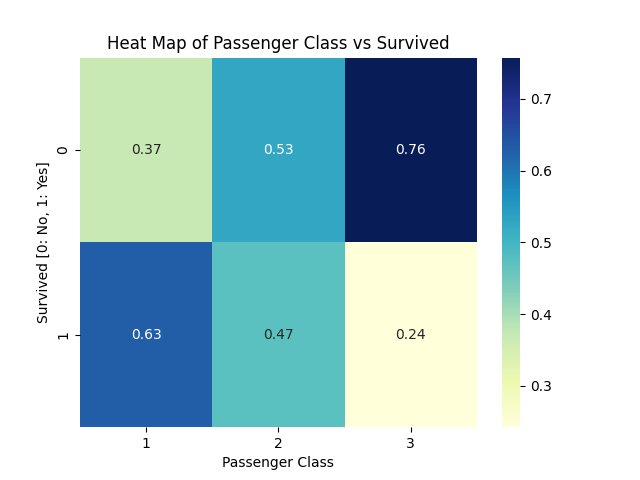
\includegraphics[width=\columnwidth]{C:/GitHub/DataScience/wk_03/plots/PClassVsSurvivedHeatMap.png}  
    \caption{Heat Map of Passenger Class vs Survived} 
\end{figure}

\subsection{Age Fill Mean vs Survived}
Now, we plot the \texttt{Age\_fill\_mean} variable against the \texttt{Survived} variable. We know that the 
\texttt{Age\_fill\_mean} is a ratio numerical data type and \texttt{Survived} is a categorical data type.
To create a plot where we plot a categorical data type against a numerical data type, we can use a violin plot, as
shown in Figure 7.

In this visualization, it appears that the meadians of both violin plots are at equal positions. The same median 
for a violin plot suggests that there is weak predictive power because the central tendency of the variable doesn't
differ significantly between the groups. As a result, this variable isn't related to the \texttt{Survived} variable.

\begin{figure}[h!] 
    \centering
    \noindent
    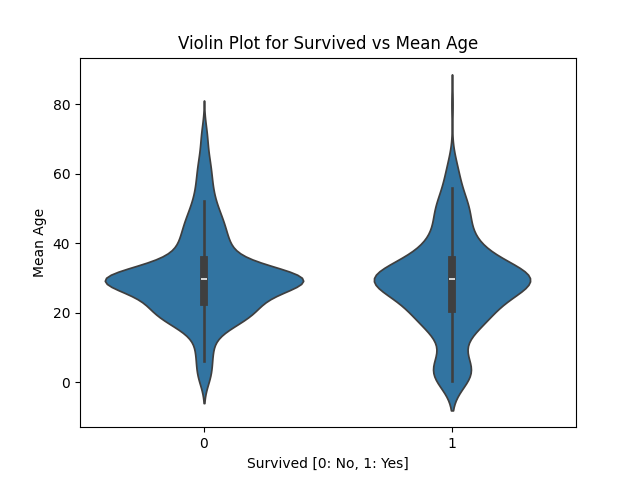
\includegraphics[width=\columnwidth]{C:/GitHub/DataScience/wk_03/plots/ViolionPlotSurvivedMean.png}  
    \caption{Violin Plot of Age (Mean) vs Survived} 
\end{figure}

\subsection{Age Fill KNN vs Survived}
Now, we plot the \texttt{Age\_fill\_KNN} variable against the \texttt{Survived} variable. We know that the 
\texttt{Age\_fill\_KNN} is a ratio numerical data type and \texttt{Survived} is a categorical data type.
To create a plot where we plot a categorical data type against a numerical data type, we can use a violin plot, as
shown in Figure 8.

In this visualization, it appears that the meadians of both violin plots are at equal positions. The same median
for a violin plot suggests that there is weak predictive power because the central tendency of the variable doesn't
differ significantly between the groups. As a result, this variable isn't related to the \texttt{Survived} variable.

\begin{figure}[h!] 
    \centering
    \noindent
    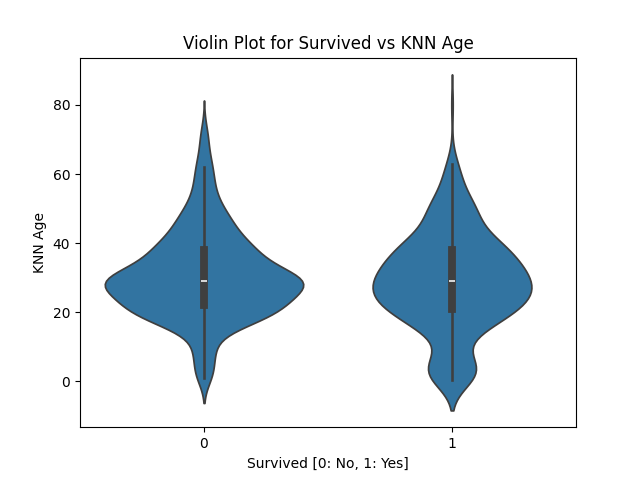
\includegraphics[width=\columnwidth]{C:/GitHub/DataScience/wk_03/plots/ViolinPlotKNNSurvived.png}  
    \caption{Violin Plot of Age (KNN) vs Survived} 
\end{figure}

\subsection{Age Fill Median vs Survived}
Next, we plot the \texttt{Age\_fill\_Median} variable against the \texttt{Survived} variable. We know that the 
\texttt{Age\_fill\_Median} is a discrete numerical data type and \texttt{Survived} is a categorical data type.
To create a plot where we plot a categorical data type against a numerical data type, we can use a violin plot, as
shown in Figure 9.

In this visualization, it appears that the meadians of both violin plots are at equal positions. The same median
for a violin plot suggests that there is weak predictive power because the central tendency of the variable doesn't
differ significantly between the groups. As a result, this variable isn't related to the \texttt{Survived} variable.

\begin{figure}[h!] 
    \centering
    \noindent
    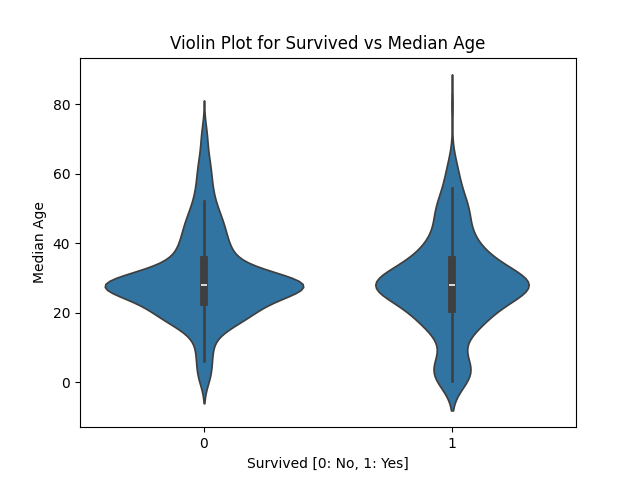
\includegraphics[width=\columnwidth]{C:/GitHub/DataScience/wk_03/plots/ViolionPlotSurvivedMedian.png}  
    \caption{Violin Plot of Age (Median) vs Survived} 
\end{figure}

\subsection{Age Fill Mode vs Survived}
Lastly, we plot the \texttt{Age\_fill\_Mode} variable against the \texttt{Survived} variable. We know that the 
\texttt{Age\_fill\_Mode} is a discrete numerical data type and \texttt{Survived} is a categorical data type.
To create a plot where we plot a categorical data type against a numerical data type, we can use a violin plot, as
shown in Figure 10.

In this visualization, it appears that the meadians of both violin plots are at equal positions. The same median 
for a violin plot suggests that there is weak predictive power because the central tendency of the variable doesn't
differ significantly between the groups. As a result, this variable isn't related to the \texttt{Survived} variable.

\begin{figure}[h!] 
    \centering
    \noindent
    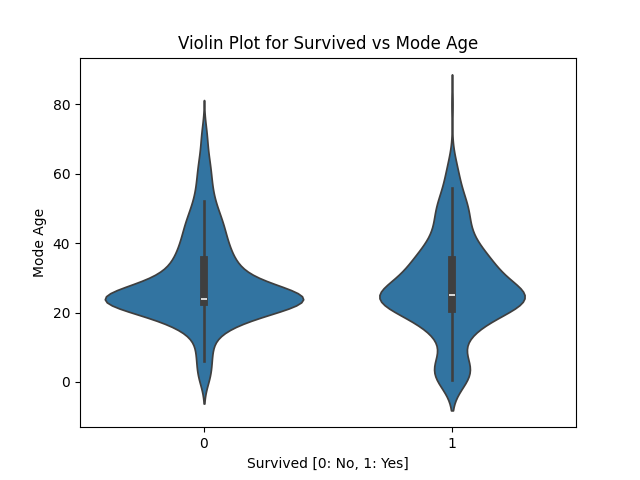
\includegraphics[width=\columnwidth]{C:/GitHub/DataScience/wk_03/plots/ViolionPlotSurvivedMode.png}  
    \caption{Violin Plot of Age (Mode) vs Survived} 
\end{figure}


\subsection{Age Fill KNN vs Fare}
Now, we plot the two features, \texttt{Age\_fill\_KNN} and \texttt{Fare} against each other using a scatterplot and
KDE Joint Plot as shown in Figures 11 and 12.

With regards to the Scatterplot, we can see that across ages from 0 to 80, the fare is quite consistent in ranging 
from 0 to 100, as the density of the points are the greatest. As a result, it is clear to say that there is no
relationship between the \texttt{Age\_fill\_KNN} and \texttt{Fare}.

With regards to the Jointplot, there is high density in the lower-left region, which is a suggestion that the 
majority of the passengers were young and had paid lower fares. Moreover, it is also evident to see that there
are some outliers, of which are mostly passengers that paid a higher fare than average. 

\begin{figure}[h!] 
    \centering
    \noindent
    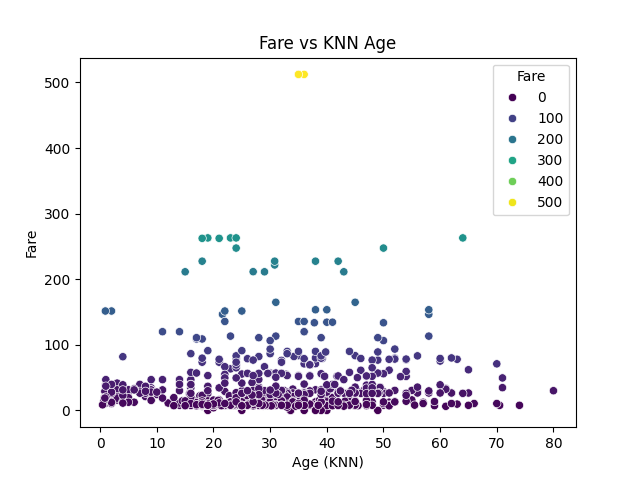
\includegraphics[width=\columnwidth]{C:/GitHub/DataScience/wk_03/plots/FareAgeKNN.png}  
    \caption{Scatterplot of Fare vs KNN Age } 
\end{figure}

\begin{figure}[h!] 
    \centering
    \noindent
    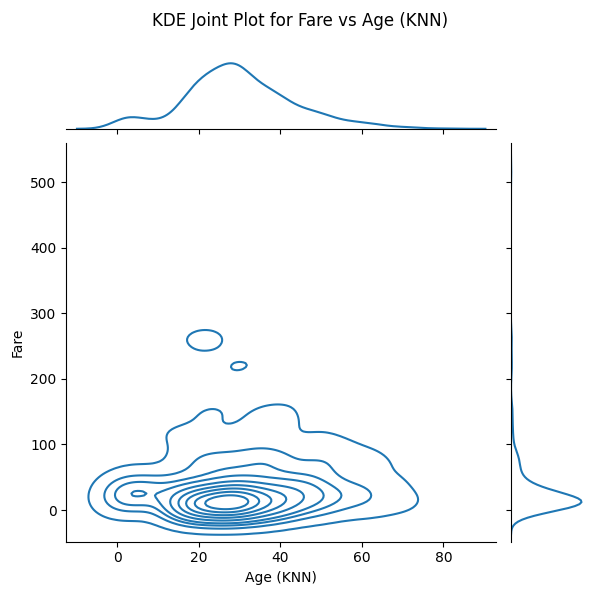
\includegraphics[width=\columnwidth]{C:/GitHub/DataScience/wk_03/plots/KDE.png}  
    \caption{KDE Joint Plot of Fare vs Age} 
\end{figure}


\section{Methods}
The different data visualizations produced spark questions with regards to how the data was handled and why it was
done in that way. We aim to justify such approaches in this section.

\subsection{Missing Values}
When we first received the titanic dataset, the \texttt{Age} feature had some empty null values. In order to deal
with such null values, we decided to perform some imputations using the mean, median, mode and producing predictive
values using a KNN model.

There are different impacts to using different methods of imputations, of which are summarized below:
\begin{enumerate}
    \item Mean: can introduce biases, which could affect the predicitve strength between \texttt{Age} and 
    \texttt{Survived}
    \item Mode: can overisimplify the data and doesn't capture the natural variation in age
    \item Median: is a good option, since it can preserve the distribution's central tendency, especially when the 
    data is skewed
    \item KNN: is a more accurate option since it uses other features in the dataset to make a prediction for 
    \texttt{age}
\end{enumerate}

As a result, the method of imputation can greatly impact the predictive relationship between \texttt{Age} and 
\texttt{Survived} because because different imputation methods affect the distribution and variance of the Age 
feature, which in turn influences the patterns we observe between Age and Survived.

\subsection{Unused Features}
It is notable to see that we haven't used the features \texttt{PassengerID} and \texttt{Cabin}. This is for the
reason that there is no relationship to be mapped out with any of the other features. It simply serves as a numbering
of each passenger and is used to check passengers in. There are too many unique values in the feature for any 
meaningful relationships to be mapped out.

However, in future, we can implement the following features in such ways:
\begin{itemize}
    \item Passenger ID: using the passenger class, we can group the passenger ID's into respective passenger classes,
    hence, we get a few unique values, thus resulting in a new feature
    \item Cabin: using the Cabin ID's, we can create a few unique values by extracting the first letter, which 
    may signify the floor level of the titanic, which in turn allows us to predict the likelihood of surviving
    on a floor of the Titanic
\end{itemize}

\subsection{Feature Selection}
Now that we have examined the relationships between all of the features, including features that we haven't
considered, it is worth discussing which features we would like to select for a machine learning model.

In order for a feature to be selected, we look for features that are meaningful and carry important information, 
such as Sex or Age. We want to avoid features that have a high correlation, such as \texttt{Age} and 
\texttt{Age\_fill\_mean}. Hence, we need to decide on which \texttt{Age} feature to choose on. Another factor that
influences the decision on choosing the \texttt{Age} feature is the type of imputation as well as having no 
missing values. 

Another reason to choose features might be the strength of the predictive relationship between them. However, there
is an argument against this. It is simply because that if a plot may appear to suggest a relationship, via, for
example, a best fit line, this necessarily does not mean it is satistically true. Another reason is that a variable's
true predictive simply lies in how much it contributes the accuracy of the model. Hence, if we were to look at such
features for a predictive relationship with \texttt{Survived}, for example, we may want to look beyond just graphs.

With the criteria set in mind, these are the following features we may choose: \texttt{Embarked}, \texttt{Pclass},
\texttt{Sex}, \texttt{Age\_fill\_Median}, \texttt{Cabin} (given that we perform string manipulation as described
in the above subsection) and \texttt{Fare}. Such features are subject to change depending on the performance of 
the model, but we choose such features due to their meaningfulness and the kinds of insights they can provide. 

\subsection{Age Fill KNN and Fare}
With regards to these features, we attempted to find any predictive relationship by using a scatterplot and a
jointplot. We can see that there is no observed relationship as we can't draw out a best fit line from the produced
scatter plot. As a result, we would not include these two correlated variables because as a result, we would not
 include these two correlated variables because their lack of a clear relationship.


\section{Results}
From the graphs that we've managed to produce, we can say that there are features that have a predictive relationship,
such as passengers of class 3 with the feature \texttt{Survived} and the same with passengers of class 1 and 2. Another
result is that we've found strong predictive features between \texttt{Embarked} where passengers who embarked from
Southampton and Queenstown were more likely to die, and passengers who embarked from Cherbourg were more likely to
survive. Lastly, there is a strong predictive relationship between the feature \texttt{Sex} where women were more 
likely to survive than men.

\section{Discussion}
Overall, this paper explored the different methods of visualizing data of different types, mainly catgorical and 
numerical. We also explored how much importance we should be placing on such visualizations and how they can be 
interpreted to give us an idea of the strength of the predictive relationship.

The visualization techniques we used give us interesting insights, such that people who emabarked from a certain
port were more likely to survive, and this inspires us to ask questions as to why? The observation that women
were more likely to survive told us that in Edwardian society that women were often given a priority in safety than
men. Furthermore, if we also look at the box plots of passengers that had children, they were also given priority. 

\end{document}
